%%%%%%%%%%%%%%%%%%%%%%%%%%%%%%%%%%%%%%%%%%
%%%%%%%%%%%%%                 %%%%%%%%%%%%
%%%%%%%%%%%%%    EXERCISE 1   %%%%%%%%%%%%
%%%%%%%%%%%%%                 %%%%%%%%%%%%
%%%%%%%%%%%%%%%%%%%%%%%%%%%%%%%%%%%%%%%%%%
\begin{exercise}[]{What protocol does "ping" and "traceroute" use?}
  \begin{solution}
  \par{~}
  ping and traceroute use ICMP(Internet Control Message Protocol). See Figure \ref{fig1}

\begin{figure}[hb]
    \begin{center}
        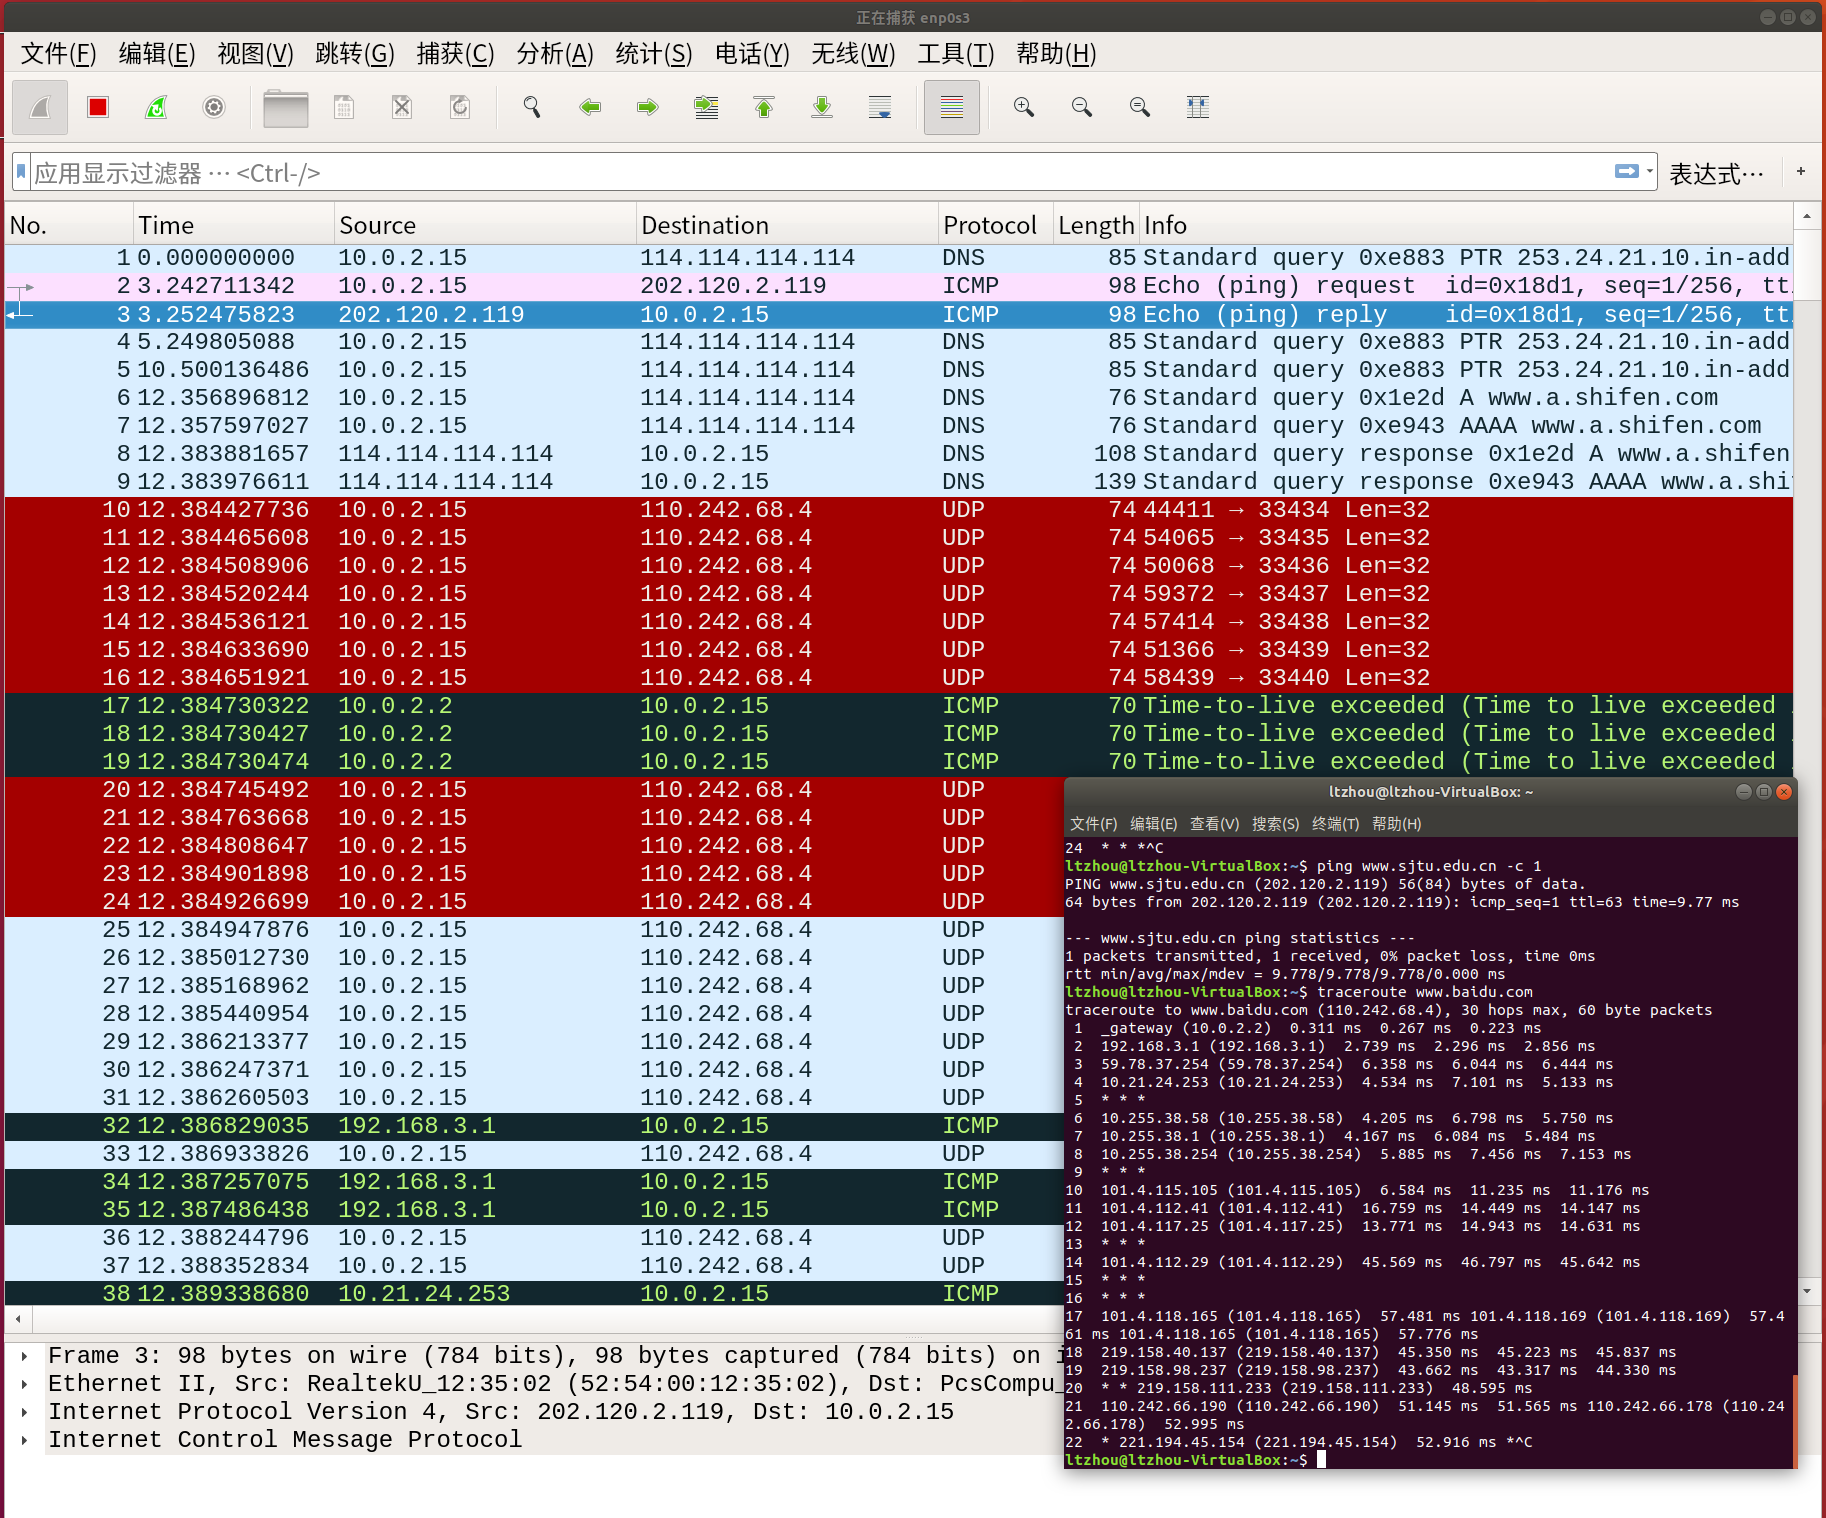
\includegraphics[width=12cm]{img/lab1/ex1}
        \caption{A ping and a traceroute command are executed in the terminal. The 2nd and 3rd record in Wireshark shows that ICMP is used in ping. The 17th - 19th record in Wireshark shows that ICMP is also used in traceroute.}
        \label{fig1}
    \end{center}
\end{figure}
  
  \end{solution}
  \label{ex1}
\end{exercise}


%%%%%%%%%%%%%%%%%%%%%%%%%%%%%%%%%%%%%%%%%%
%%%%%%%%%%%%%                 %%%%%%%%%%%%
%%%%%%%%%%%%%    EXERCISE 2   %%%%%%%%%%%%
%%%%%%%%%%%%%                 %%%%%%%%%%%%
%%%%%%%%%%%%%%%%%%%%%%%%%%%%%%%%%%%%%%%%%%
\begin{exercise}[]{What is the IP address of www.sjtu.edu.cn? }
  \begin{solution}
  \par{~} From my experiment, IP address of www.sjtu.edu.cn is 202.120.2.119

  \begin{figure}[h]
    \begin{center}
    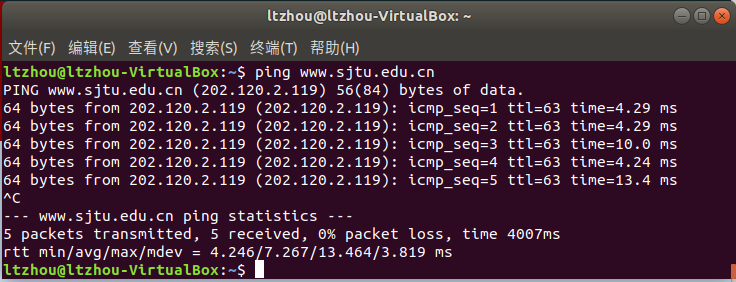
\includegraphics[width=12cm]{img/lab1/ex2}
    \caption{The IP address is obtained by pinging the domain name of SJTU}
    \label{fig:ex2}
    \end{center}
  \end{figure}
  \end{solution}
  \label{ex2}
\end{exercise}

\newpage

%%%%%%%%%%%%%%%%%%%%%%%%%%%%%%%%%%%%%%%%%%
%%%%%%%%%%%%%                 %%%%%%%%%%%%
%%%%%%%%%%%%%    EXERCISE 3   %%%%%%%%%%%%
%%%%%%%%%%%%%                 %%%%%%%%%%%%
%%%%%%%%%%%%%%%%%%%%%%%%%%%%%%%%%%%%%%%%%%
\begin{exercise}[]{What is the average round trip time (RTT) from your VM to www.sjtu.edu.cn and mit.edu.
    Analyze the reason for the difference of their RTTs.}
  \begin{solution}
  \par{~}
  RTT for www.sjtu.edu.cn is 7.706 ms on average. RTT for mit.edu is 214.188 ms on average. More details can be found in Figure \ref{fig:ex3}.

  The reason why RTT for mit takes longer than that for SJTU is probably because in order to reach the host in MIT, the packet has to travel through more routers, thus increasing transmission delay, queuing delay, etc.

  \begin{figure}[hb]
    \begin{center}
    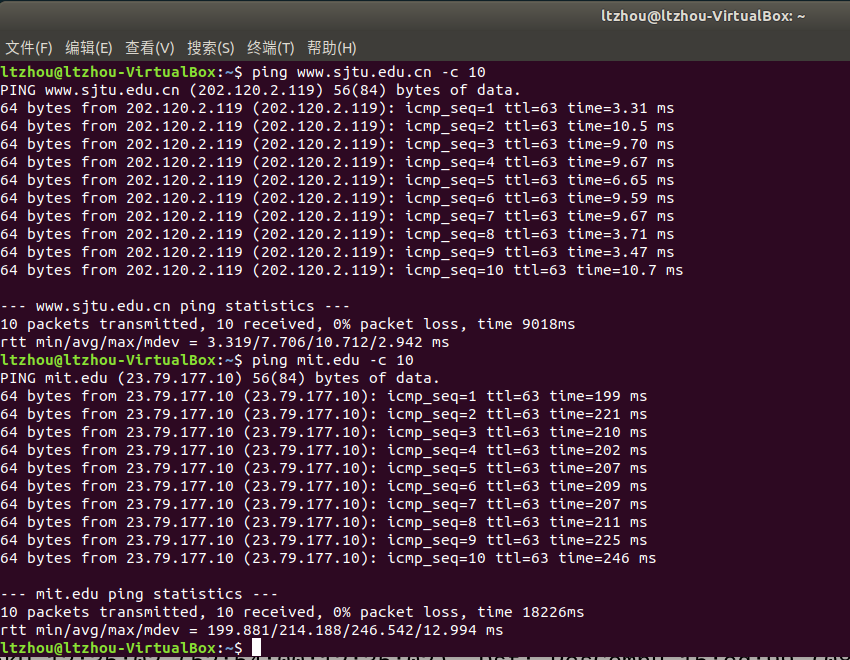
\includegraphics[width=12cm]{img/lab1/ex3}
    \caption{10 packets are sent by the ping command for each site}
    \label{fig:ex3}
    \end{center}
  \end{figure}
  \end{solution}
  \label{ex3}
\end{exercise}


%%%%%%%%%%%%%%%%%%%%%%%%%%%%%%%%%%%%%%%%%%
%%%%%%%%%%%%%                 %%%%%%%%%%%%
%%%%%%%%%%%%%    EXERCISE 4   %%%%%%%%%%%%
%%%%%%%%%%%%%                 %%%%%%%%%%%%
%%%%%%%%%%%%%%%%%%%%%%%%%%%%%%%%%%%%%%%%%%
\begin{exercise}[]{What is the TCP bandwidth between your two VMs?}
  \begin{solution}
  \par{~}
  The bandwidth between two VMs are about 4 Gbits/sec, shown in Figure \ref{fig:ex4}
  \begin{figure}[hb]
    \begin{center}
    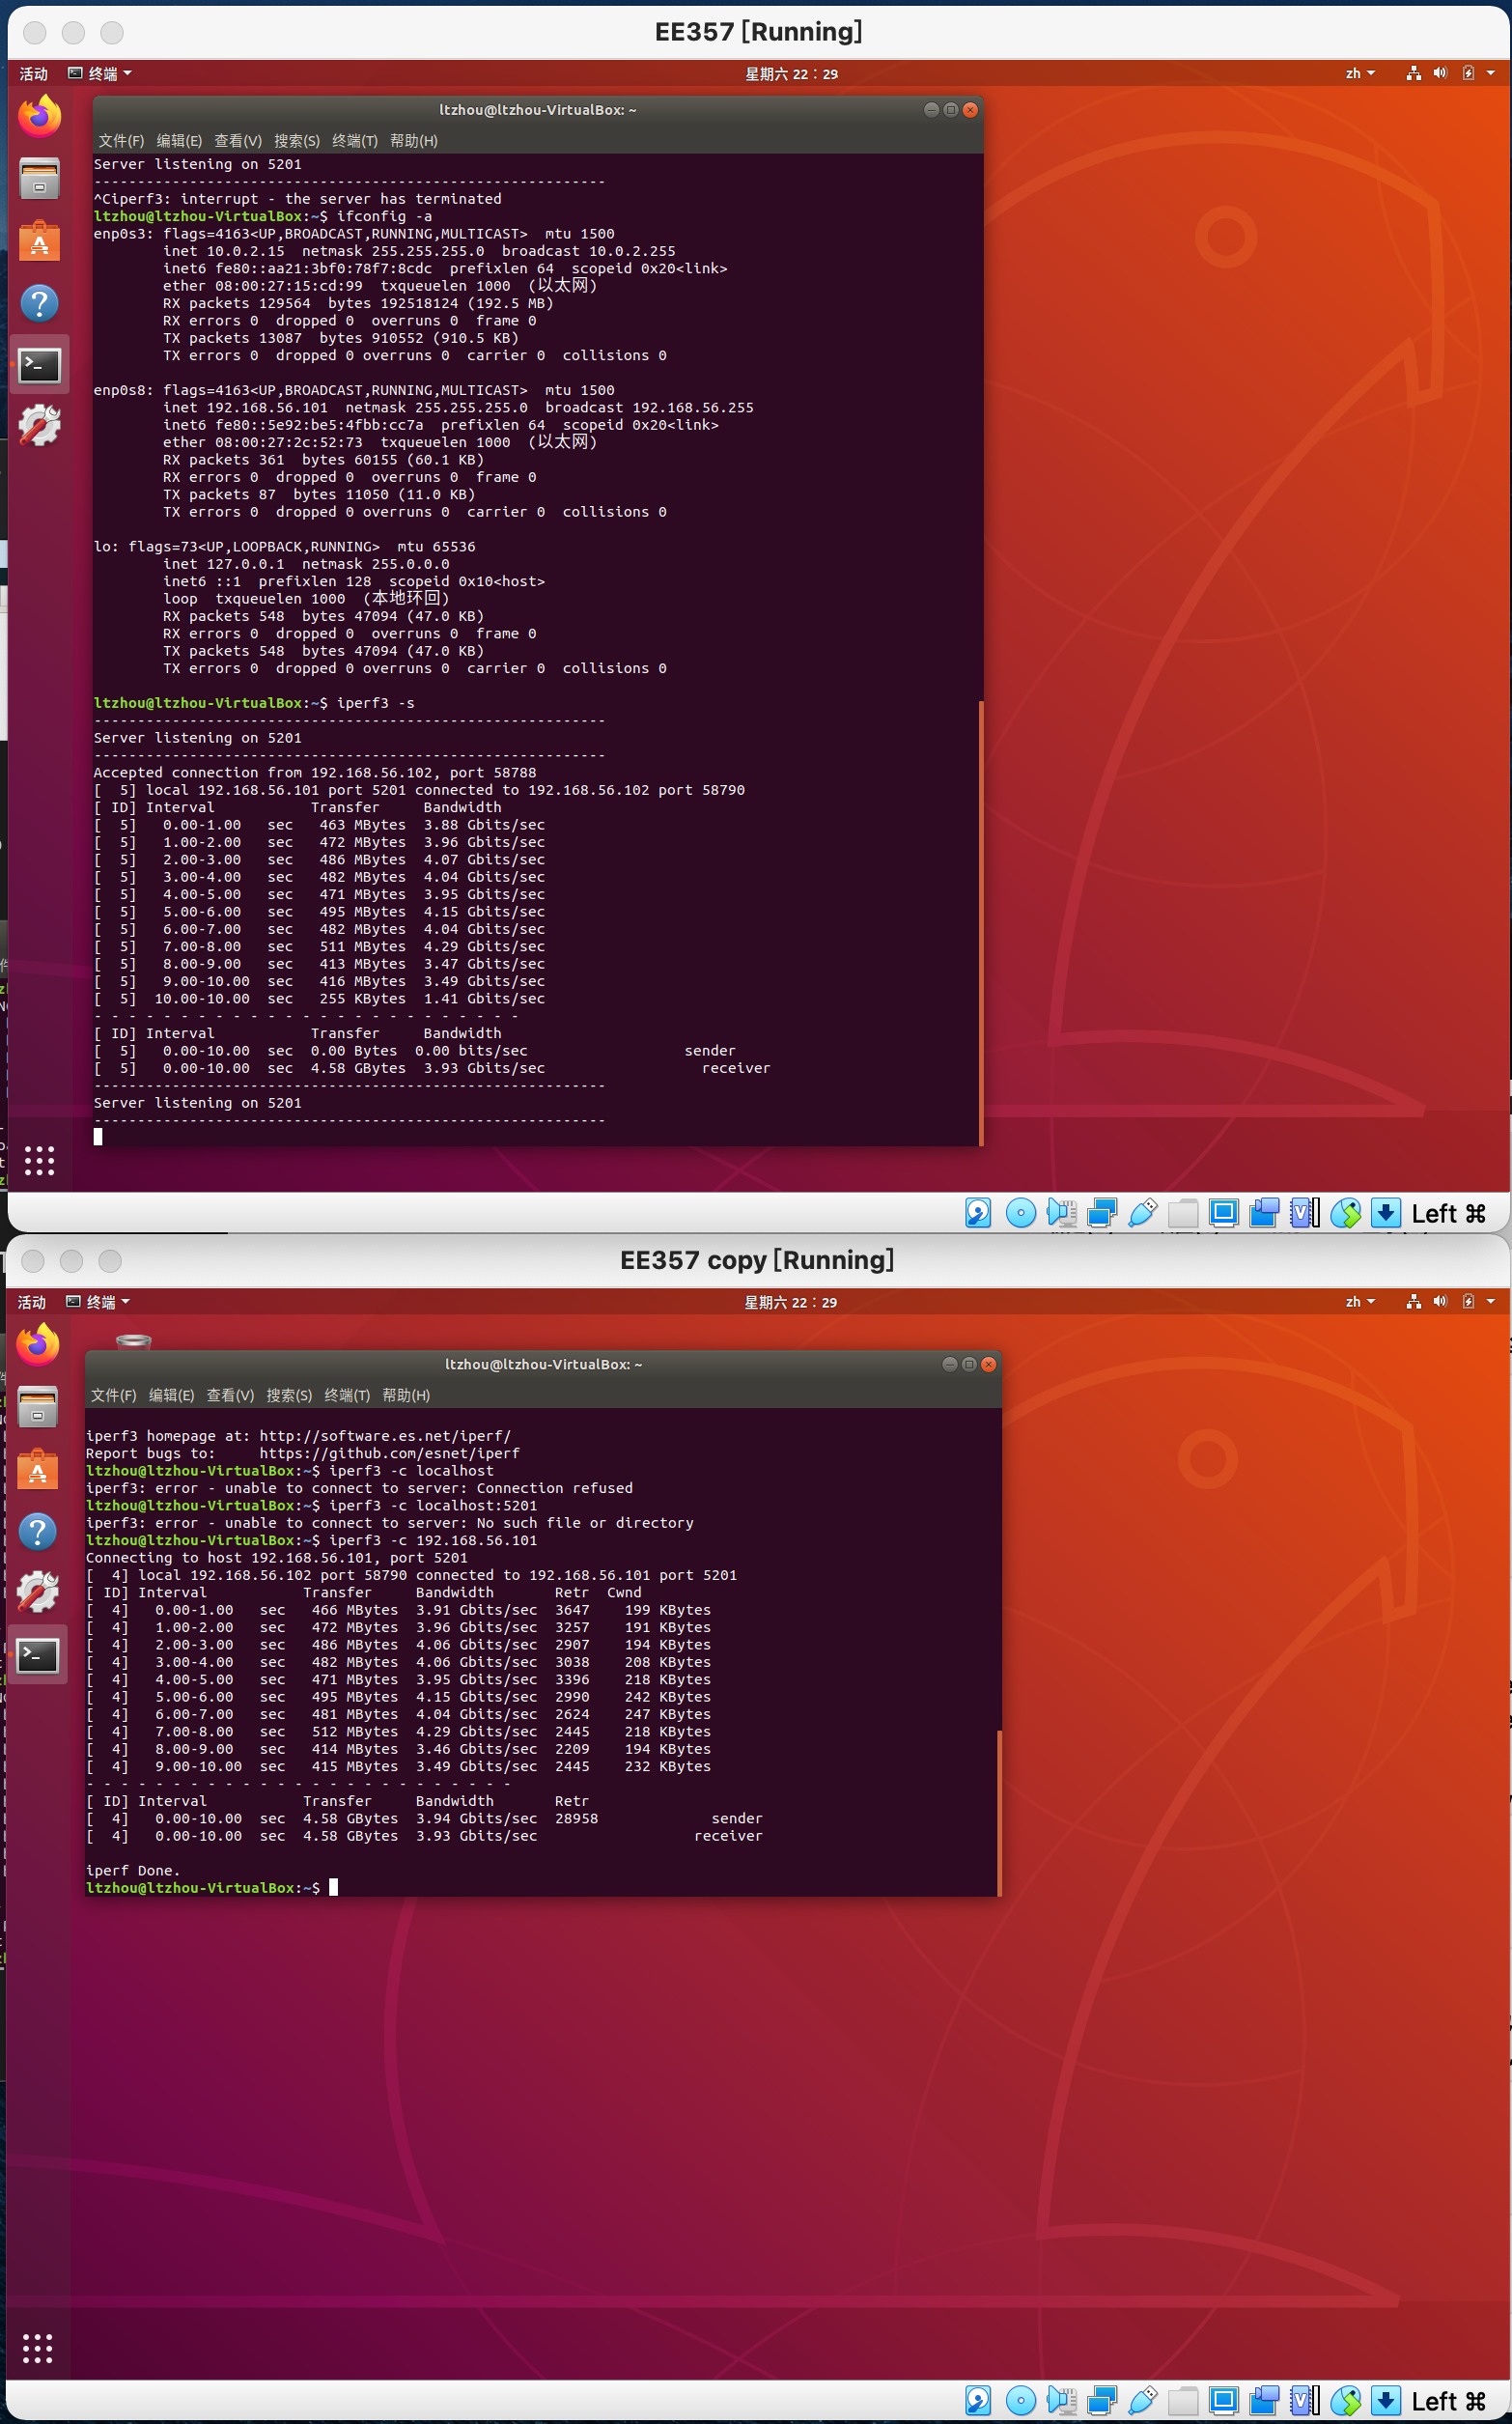
\includegraphics[width=12cm]{img/lab1/ex4}
    \caption{Use iperf to test TCP bandwidth between two VMs. The above VM is the server, and the below is host}
    \label{fig:ex4}
    \end{center}
  \end{figure}
  \end{solution}
  \label{ex4}
\end{exercise}


%%%%%%%%%%%%%%%%%%%%%%%%%%%%%%%%%%%%%%%%%%
%%%%%%%%%%%%%                 %%%%%%%%%%%%
%%%%%%%%%%%%%    EXERCISE 5   %%%%%%%%%%%%
%%%%%%%%%%%%%                 %%%%%%%%%%%%
%%%%%%%%%%%%%%%%%%%%%%%%%%%%%%%%%%%%%%%%%%
\begin{exercise}[]{Select a VM as your host machine, and another VM as your server machine, then use ssh on your host to connect to the server.}
  \begin{solution}
  \par{~} See Figure \ref{fig:ex5}
  \begin{figure}[hb]
    \begin{center}
    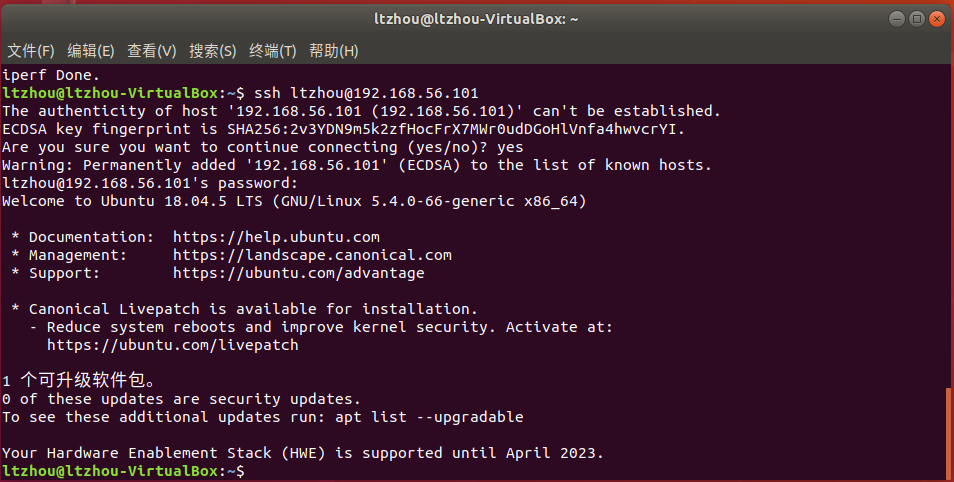
\includegraphics[width=12cm]{img/lab1/ex5}
    \caption{ssh screenshot}
    \label{fig:ex5}
    \end{center}
  \end{figure}
  \end{solution}
  \label{ex5}
\end{exercise}

%%%%%%%%%%%%%%%%%%%%%%%%%%%%%%%%%%%%%%%%%%
%%%%%%%%%%%%%                 %%%%%%%%%%%%
%%%%%%%%%%%%%    EXERCISE 6   %%%%%%%%%%%%
%%%%%%%%%%%%%                 %%%%%%%%%%%%
%%%%%%%%%%%%%%%%%%%%%%%%%%%%%%%%%%%%%%%%%%


\begin{figure}[hb]
  \begin{center}
  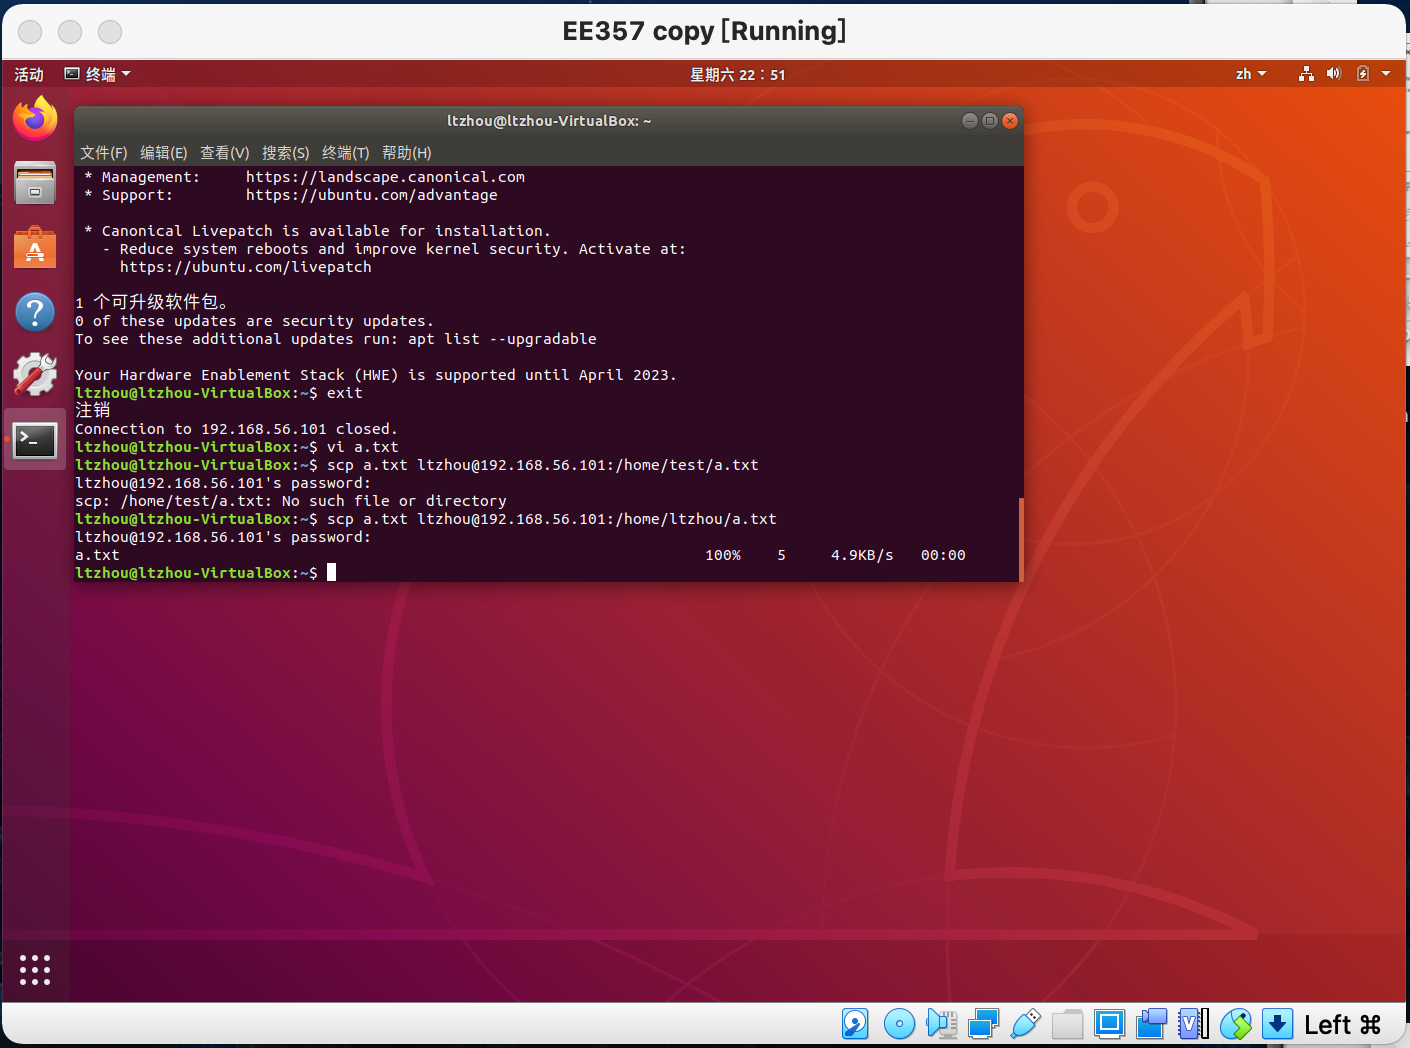
\includegraphics[width=12cm]{img/lab1/ex6-2}
  \caption{“a.txt” is created in the host machine, it is copied to the “/home/ltzhou directory of the server machine}
  \label{fig:ex61}
  \end{center}
\end{figure}

\begin{figure}[hb]
  \begin{center}
  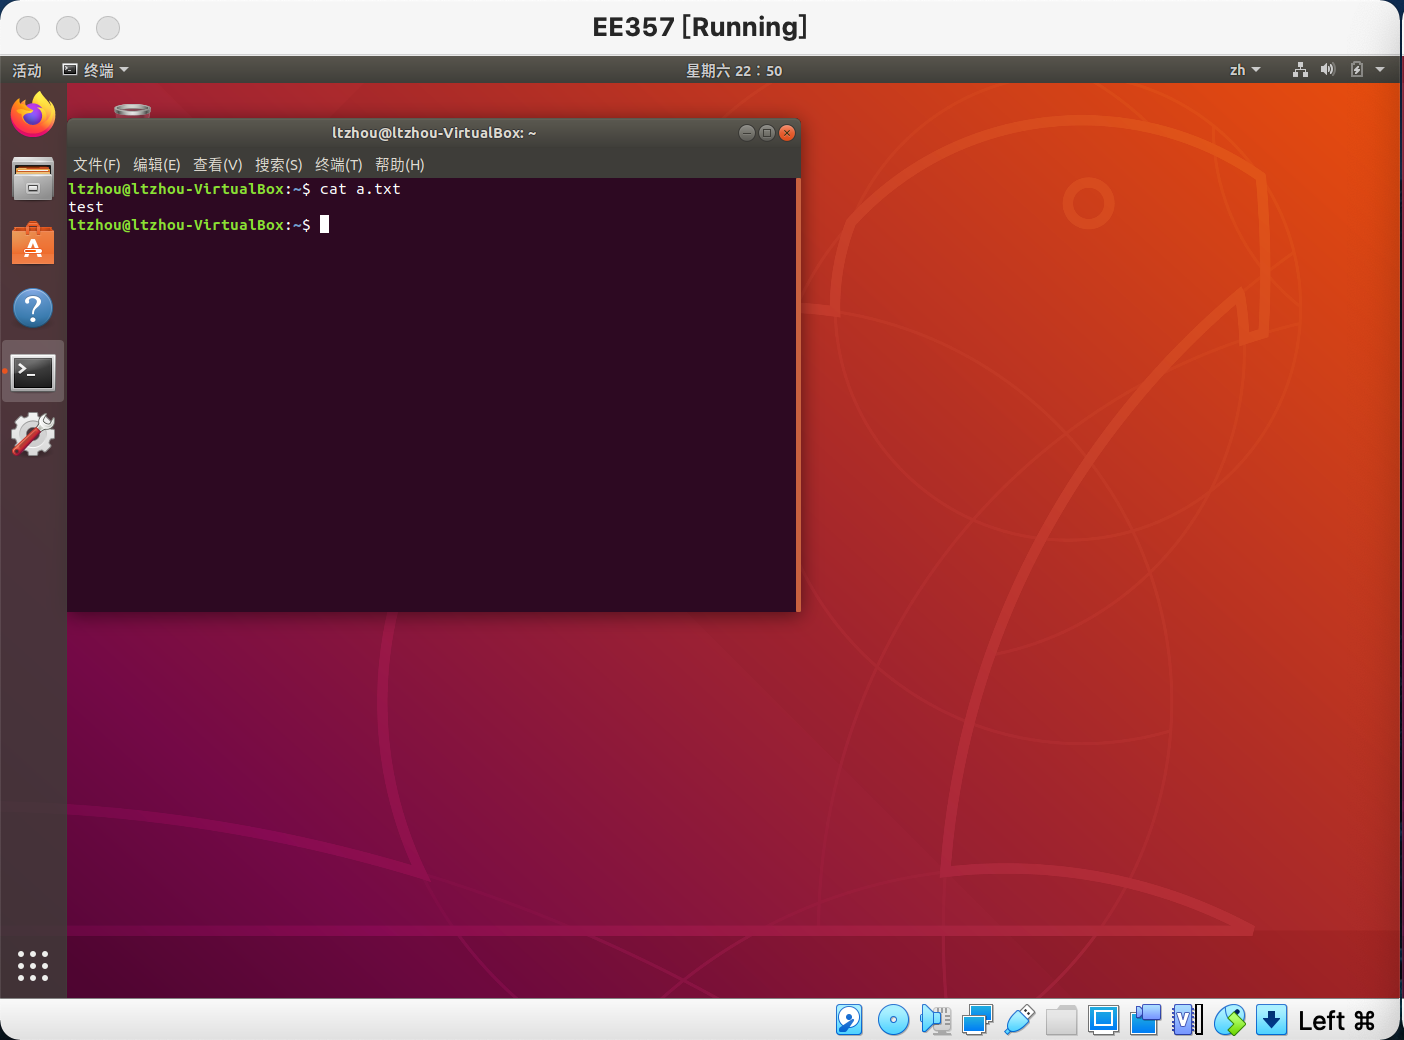
\includegraphics[width=12cm]{img/lab1/ex6-1}
  \caption{"a.txt" is transferred to the server machine}
  \label{fig:ex62}
  \end{center}
\end{figure}

\begin{exercise}[]{Use scp to copy a file from your host to the server.}
  \begin{solution}
  \par{~}
  See Figure \ref{fig:ex61}, Figure \ref{fig:ex62}.

  \end{solution}
  \label{ex6}
\end{exercise}
